\subsubsection{Overview}
The Actor will be responsible for simulating the execution of the solution constructed
by the player through movement and animations. It is an animated character in the game that will move around the Puzzle Scene and manipulate the data elements of the current puzzle based on the sequence of commands that the player constructs in the Solution Pane of the User Interface. \\

Figure \ref{fig:actor_diagram} provides a high-level outline of the Actor component, all of its internal processes, and how it interacts with the other core aspects of the game.\\

\begin{figure}[!htb]
  \caption{Actor Component Overview}
  \label{fig:actor_diagram}
  \centering
  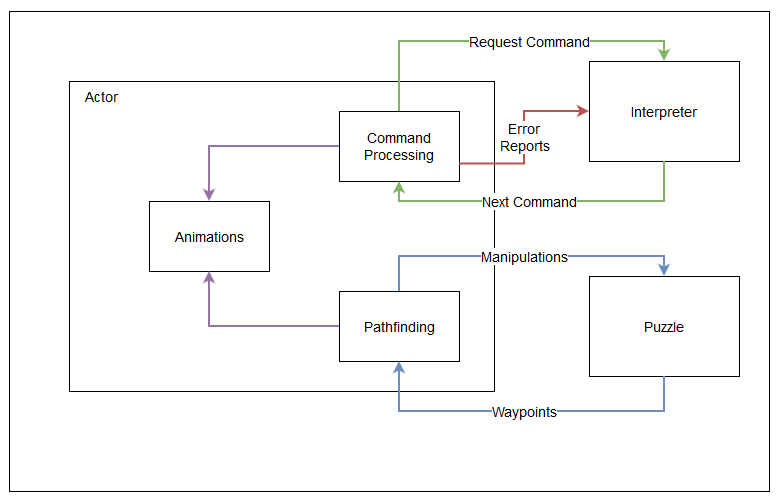
\includegraphics[scale=0.8]{Diagrams/actor_diagram.png}
\end{figure}
\newpage
The responsibilities of the Actor are as follows:

\begin{itemize}
	\item Retrieve commands from the Interpreter component
	\item Alert the Interpreter component to halt execution when an invalid command is attempted
	\item Move to the correct waypoints based on the command received
	\item Properly handle data manipulation in the puzzle scene (move and update data elements
			as specified by the current command)
	\item Communicate the flow of execution to the player through animations
	\item Illustrate to the player how data changes in response to commands via animations
	\item Tell the player about runtime errors in their code
\end{itemize}

\subsubsection{Interpreter Interactions}
Effective integration with the Interpreter is a key component of the functionality of the Actor. The Actor relies completely on the command sequence from the Interpreter in order to illustrate the execution of the solution. The Actor will continue to retrieve the next command in sequence from the Interpreter until the sequence terminates or an invalid command is attempted. If the command can be executed, the Actor will carry out the instruction visually so that the player can understand the flow of execution and the logic behind their solution. If the command causes an error in execution, the Actor will alert the Interpreter to halt execution. The flow of this process between the Actor and Interpreter can be seen in Figure \ref{fig:interpreter_interactions}.\\

\begin{figure}[!htb]
  \caption{Interactions between the Interpreter and Actor components}
  \label{fig:interpreter_interactions}
  \centering
  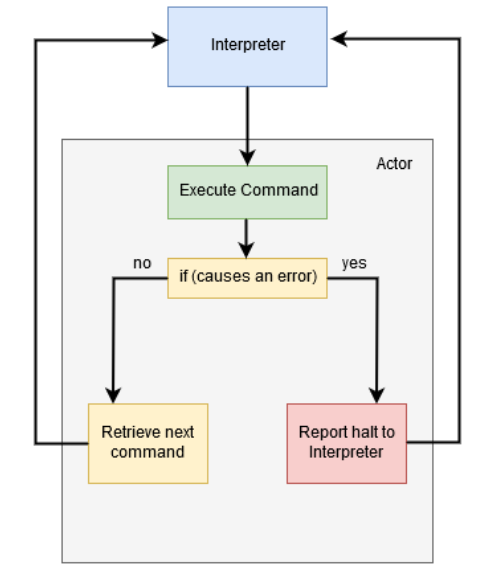
\includegraphics[scale=0.8]{Diagrams/interpreter_interactions.png}
\end{figure}

As mentioned in Section 6.5.4, there is a three step handshake between the Actor and the Interpreter when processing instructions. To summarize, the Actor requests the next command, the Interpreter responds with a data structure of that command, and the Actor then reports the results of the execution of that command to the Interpreter. Again, this communication flow can be seen in Figure \ref{fig:interpreter_Actor_interface}. 

\subsubsection{Processing Commands}
The processing of commands is the core function of the Actor. Interfacing with the Interpreter component is only the first part of command processing; the majority of that processing occurs independently within the Actor component once a command has been retrieved. Figure \ref{fig:processing_commands} shows in detail how the Actor internally processes commands.\\

\begin{figure}[!htb]
  \caption{The state diagram followed by the actor when processing commands}
  \label{fig:processing_commands}
  \centering
  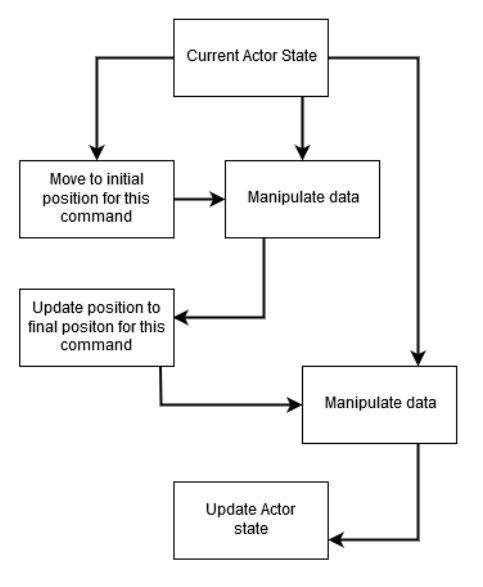
\includegraphics[scale=0.8]{Diagrams/processing_commands.png}
\end{figure}

After fetching a command, the Actor will then execute a series of movements and actions to carry out that command. This includes moving to the proper waypoint to initiate the instruction, manipulating data from the Puzzle Scene object the Actor is currently at, moving to a second waypoint to continue execution, and manipulating data at that second Puzzle Scene object. Depending on what the current command is and the status of the actor when the new command is retrieved, some of these four steps may not be applicable. Parsing each instruction separately and successfully regardless of the current state is vital. Commands that cause errors must be reported accurately back to the Interpreter so that execution can be halted when they are encountered, and no false reporting can be tolerated. If the command won't cause an error until it is partially completed, the partial execution of that command must be shown. Additionally, commands that can complete without causing errors should always be carried out exactly as specified. This is integral to the process of the game because even if the command is the wrong selection at the time, it still needs to be executed properly in the puzzle to show the player the error in their logic. Of course, correct commands that work towards the solution also need to be executed properly to eventually reach the solved state of the puzzle.\\

The command passed from the Interpreter to the Actor needs to have several fields:
\begin{itemize}
	\item Command Opcode
	\item Command Argument
	\item Success Indicator
	\item Evaluation Indicator
\end{itemize}
The associated opcode for the command is a an integer value unique to that command. Each command in the language has a corresponding opcode. By reading these values, the Actor will know which instruction type it needs to process. The argument for that command will provide additional information to the Actor, such as which Memory Card the Actor will be interacting with when it is processing a command at the Registers Waypoint. The success indicator is a validation variable that will indicate whether or not the command was executed successfully. These first three fields are part of every command within the language of our game; the final field, however, is only required for those commands that require something to be evaluated. Specifically, the conditional jump commands. These commands dictate the control of execution based on their results, and so the result of the evaluation -- true or false -- needs to be reported back to the Interpreter so that it knows which instruction in the solution should receive the control of execution next. For this reason, these commands have been packaged in a struct (as seen in Figure \ref{fig:command_struct} that will be passed by reference to the Actor for modification as it executes the command so that the Interpreter can see updates in real time and respond accordingly to halts in execution or changes in control of execution.\\


\begin{figure}[!htb]
  \caption{The form of the struct used for packaging the fields of the Command}
  \label{fig:command_struct}
  \centering
  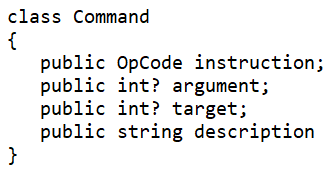
\includegraphics{command_struct.png}
\end{figure}

\subsubsection{Player Messaging}
The Actor is also a key component of communication with the player. Through the visual execution of the instructions that the player has selected, the Actor conveys how the solution the player built functions. This includes not just moving around the board and manipulating the data elements, but also providing visual cues to the user via detailed animations. For example, the data elements will be visibily picked up and held by the Actor. If that data is copied to another location, the Actor will be seen producing a copy of that data and placing it at the location specified. Data that is incremented or decremented via commands will be changed according to those commands so that the player sees and understands how the data elements are being manipulated. Additionally, providing expressive and emotive animations enhances the clarity of communication without bogging down the player with too much text. If the current command is to select the next element from Input but the Input box is empty, the Actor would attempt to pick up the item, find that nothing is there, and then emphasize that their hands are empty.\\

Aside from effective visual communication, the Actor will also provide information to the player via text when applicable. For the most part, this will be explicitly in response to runtime errors that are encountered during execution. Because a certain runtime error is always the same no matter what instance of the attempted puzzle solution causes it to occur, the Actor can provide messaging prompts to the player about these errors independently of the puzzle itself. As previously seen in Figure \ref{fig:processing_commands}, the Actor processes the success of commands completely independently and reports those errors back to the Interpreter so that the Interpreter can halt execution. It is because of this independent evalution that the Actor does not need to rely on input from any other systems in order to provide successful messaging on these errors.\\

In addition to error messaging, the Actor can also give messaging prompts to the player based on certain conditions. For example, the Actor may give an encouraging message from a random bank when a puzzle is successfully solved. This form of communication will be used sparingly and will always be coupled with visual cues to help cut down on the amount of explicit text required to convey the information to the player. Because the Actor is essentially the only character in the game as well as the focus of the game action, any dynamic messaging that needs to occur will come from the Actor. Based on the success status of the execution of certain commands, the Actor will access appropriate messaging from a bank in the Message Center to display as output, as seen in Figure \ref{fig:actor_messaging}. Static messaging that does not change based on current activity will be left to the User Interface.\\

\begin{figure}[h]
  \caption{The Message Center of the Actor}
  \label{fig:actor_messaging}
  \centering
  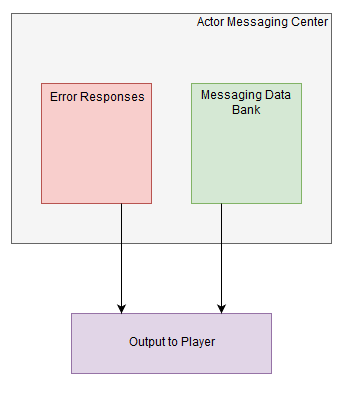
\includegraphics{actor_messaging.png}
\end{figure}